% !TeX root = ../../main.tex
% Add the above to each chapter to make compiling the PDF easier in some editors.

\chapter{Introduction}\label{chapter:introduction}

Reinforcement learning \textbf{(RL)}~\ref{fig:rl} is an area of machine learning~\ref{fig:rl_2} inspired by behaviorist psychology and intersect between different fields including neuroscience, psychology, mathematics and economics~\ref{fig:rl_1}. It has revolutionized our understanding of learning in the brain over the last 20 years. Unlike other machine learning approaches, that are dependent on \textit{pre-collected data}, Reinforcement Learning allows an agent to take actions to observe and interact with an environment to maximize total rewards towards achieving specific goals.

\begin{figure}[!htb]
		\centering
		\begin{subfigure}[b]{0.4\textwidth}
				\centering
				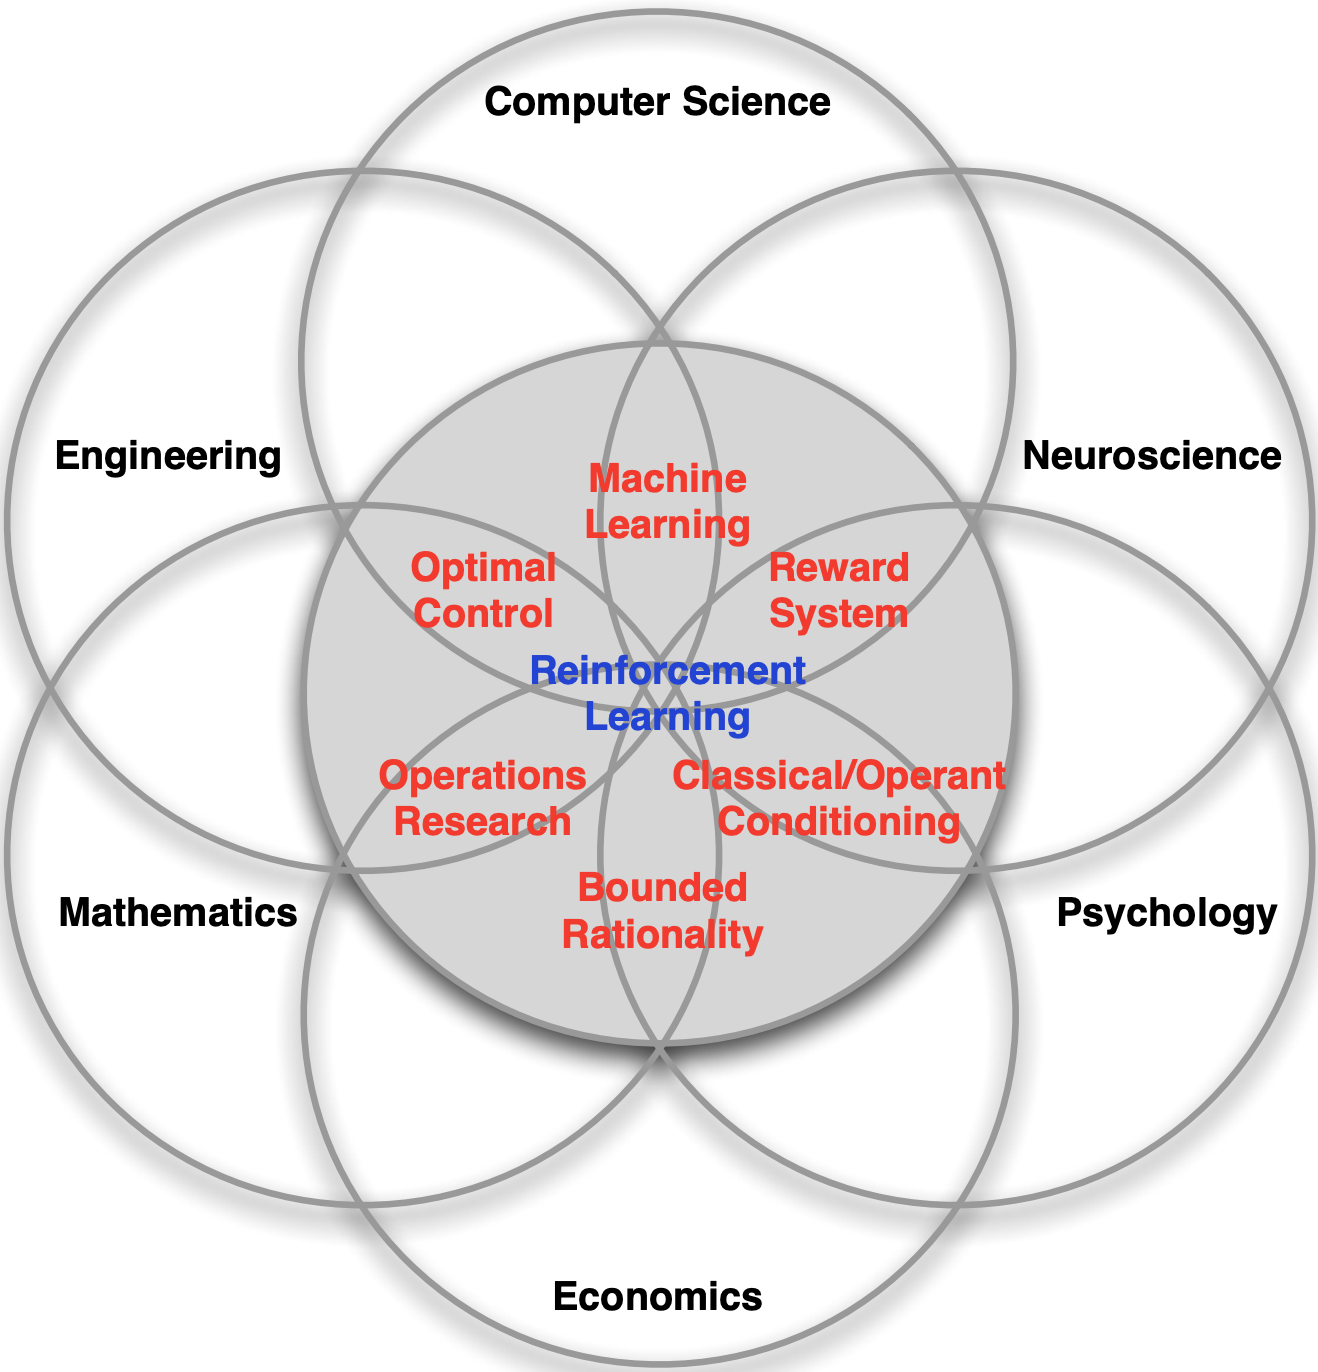
\includegraphics[width=\textwidth]{figures/rl/rl_1.png}
				\caption{Faces of Reinforcement Learning}
				\label{fig:rl_1}
		\end{subfigure}
		\hfill
		\begin{subfigure}[b]{0.4\textwidth}
				\centering
				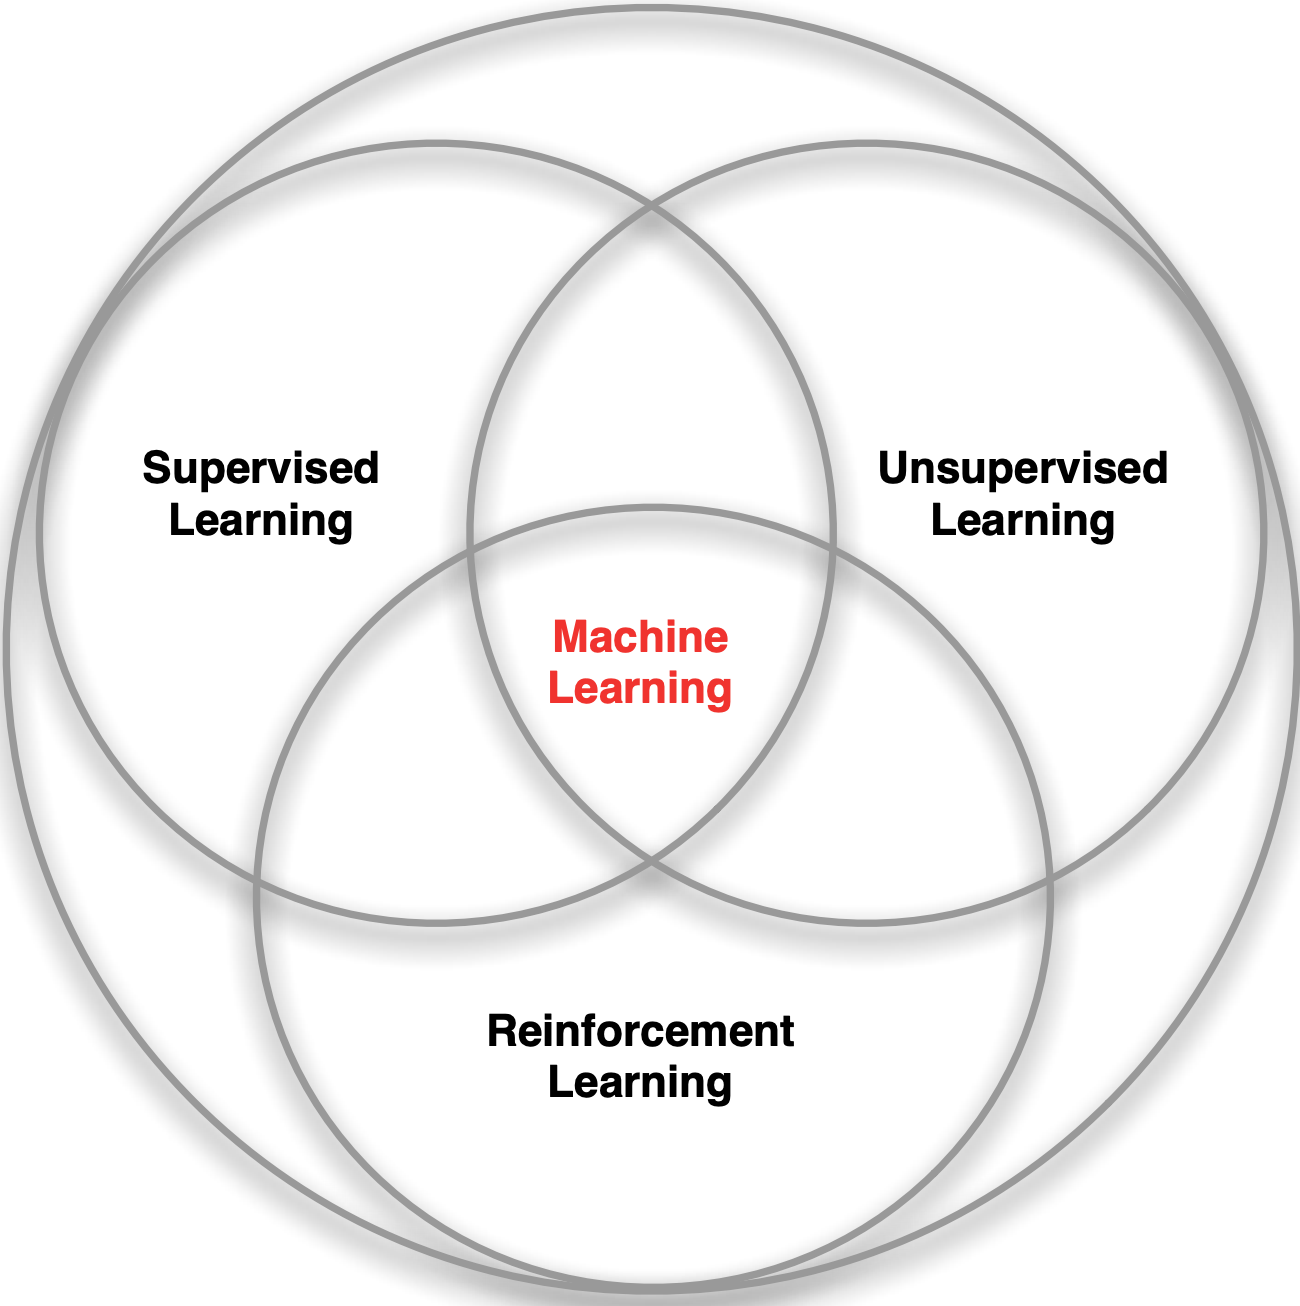
\includegraphics[width=\textwidth]{figures/rl/rl_2.png}
				\caption{Branches of Machine Learning}
				\label{fig:rl_2}
		\end{subfigure}
		\hfill
		 \caption{General Overview of Reinforcement Learning~\parencite{deepmind_rl}}
		 \label{fig:rl}
\end{figure}


Reinforcement learning combined with deep learning offers a promising path within the study of intelligent systems for achieving Artificial General Intelligence, which mimics the human's ability to learn from its own experiences. It is best applied to situations where algorithms have to decide according to their environment.

Artificial General Intelligence \textbf{(AGI)} is a type of \textit{\textbf{meta-learning}} introducing one concept where a machine can successfully understand, learn and perform any intellectual task that a human being can and the ability to learn multiple tasks, allowing the machine to \textit{learn how to learn and generalize it to acquire new skills, the way humans do}. Hence, AGI focuses on the study of systems that can perform tasks successfully across different problem domains. Most of the current ``conventional'' AI systems are domain-specific. General problem-solving ability is one that humans naturally exhibit along with decision making under uncertainty, which provides a generalization to facilitates broad situation inference.
Reinforcement Learning may pave the way for a breakthrough in our ability to build systems that will eventually exhibit human-level intelligence.

Over the past few years, reinforcement learning approaches have many interesting applications and advancements which achieved remarkable results in many areas. Starting from playing atari games and achieving human-level performance~\parencite{mnih2015human} to defeating champions of chess, shogi and Go~\footnote{\textit{In The game of Go, The number of possible configurations of the board is more than the number of atoms in the universe}} with \textbf{Deepmind's AlphaGo Zero}~\parencite{silver2017mastering}, followed by defeating the world's top players in the game of DOTA 2~\footnote{\textit{DOTA 2: a real-time strategy game, one of the most popular and complex esports games in the world which has an infinite number of states and gameplay}} with \textbf{OpenAI FIVE}~\parencite{OpenAI_dota}. Moreover, Reinforcement learning have been used for complex tasks and sequential decision making in unknown environments which is very useful for complex applications and fields like \textit{robotics}~\parencite{kober2013reinforcement, levine2016end, 45926, singh2019end}, \textit{autonomous driving}~\parencite{sallab2017deep, xu2018zero}, \textit{web system configurations and telecommunication}~\parencite{bu2009reinforcement}, \textit{computer clusters resources management}~\parencite{mao2016resource}, \textit{traffic light control}~\parencite{arel2010reinforcement}, and \textit{chemistry}~\parencite{zhou2017optimizing}.

\section{Motivation}

Reinforcement learning has achieved groundbreaking results leading the way to the best intelligent systems we could ever have.
However, since the current techniques and algorithms deal with learning to continuously operate within an uncertain environment based on delayed and limited feedback, this requires huge amount of training data to be able to learn a policy —a mapping from the state of the environment to a choice of action— that yields effective performance over time.

Despite the training data usually get collected ``on the fly'' while training as the agent starts with no prior knowledge of the environment and then starts collecting experiences through interacting with the environment, it still takes time to collect and store data, pass it to the algorithm to get updated and enhance the performance of the agent. This leads the training process to take many hours, days or even weeks for some complex algorithms and systems. Nevertheless, it requires an enormous amount of computing power to achieve the desired results. 

Following an illustration~\ref{fig:zero_and_five} of two examples for two of the most successful and breakthrough advancements in Reinforcement Learning field, to demonstrate the training time and huge computation power to train such algorithms.

\textbf{Deepmind's AlphaZero}~\parencite{silver2017mastering} starts learning by playing games against itself, starting from completely random play. The neural network in AlphaGo Zero is trained from games of self-play by a novel reinforcement learning algorithm along with Monte-Carlo Tree Search (MCTS)~\ref{fig:alphago_search_tree}. 
Despite AlphaGo Zero used a single machine with \textit{4 tensor processing units (TPUs)}, in contrast with AlphaGo that was distributed over many machines and used \textit{48 TPUs}, it still took \textbf{21 days} it surpasses AlphaGo Master and \textbf{40 days}~\ref{fig:alphago_train} to surpass all other versions of AlphaGo.

\textbf{OpenAI FIVE}~\parencite{OpenAI_dota} plays 180 years worth of games against itself every day, learning via self-play. It trains using a scaled-up version of Proximal Policy Optimization running on \textbf{256 GPUs and 128,000 CPU cores}~\ref{fig:five_hardware}.

This illustrations~\ref{fig:zero_and_five} show the amount of time along with computation and power consumptions required by the two algorithms to master the assigned tasks and get desired results. 

\begin{figure}[!htb]
		\centering
		\begin{subfigure}[b]{0.3\textwidth}
				\centering
				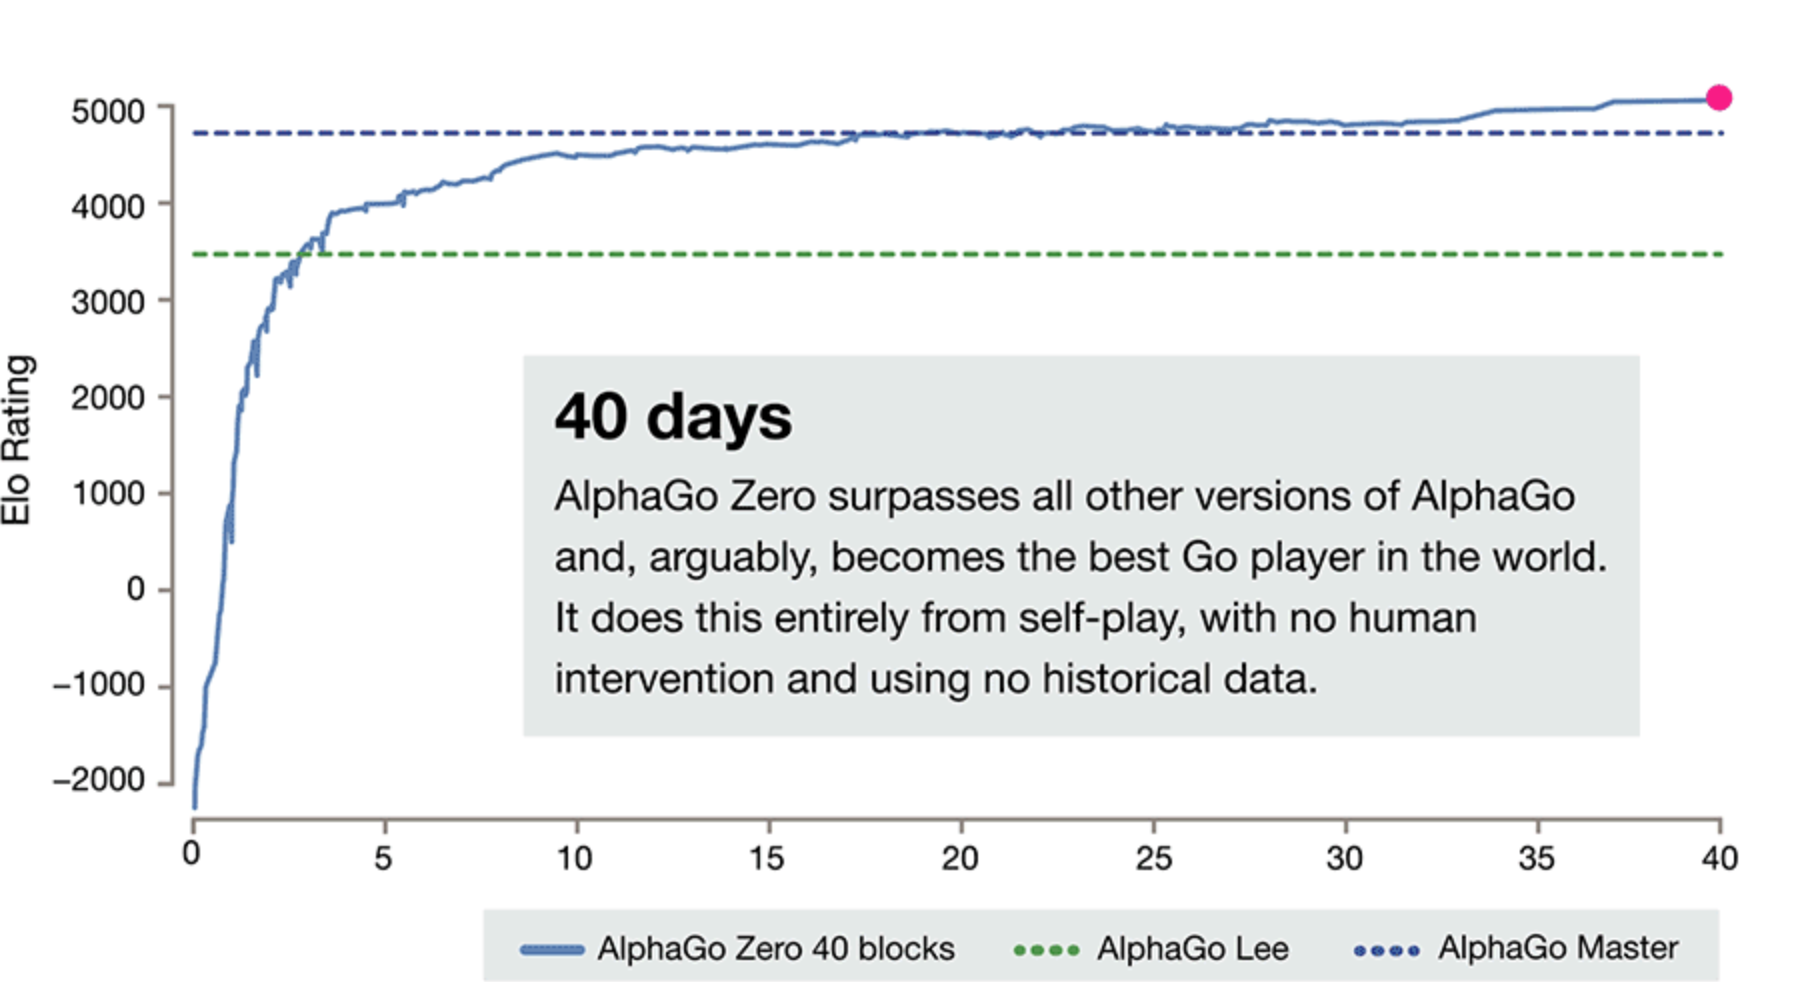
\includegraphics[width=\textwidth]{figures/rl/alphago_zero.png}
				\caption{AlphaGo Zero Training Time}
				\label{fig:alphago_train}
		\end{subfigure}
		\hfill
		\begin{subfigure}[b]{0.3\textwidth}
				\centering
				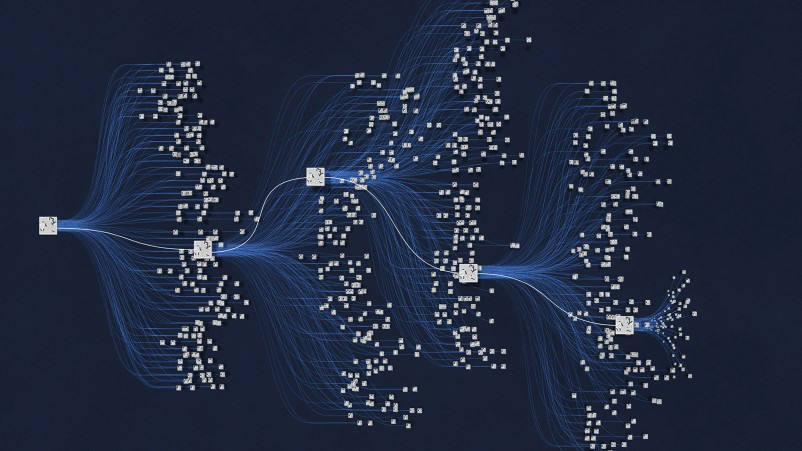
\includegraphics[width=\textwidth]{figures/rl/alphago_search_tree.png}
				\caption{AlphaGo Search Tree}
				\label{fig:alphago_search_tree}
		\end{subfigure}
		\hfill
		\begin{subfigure}[b]{0.3\textwidth}
				\centering
				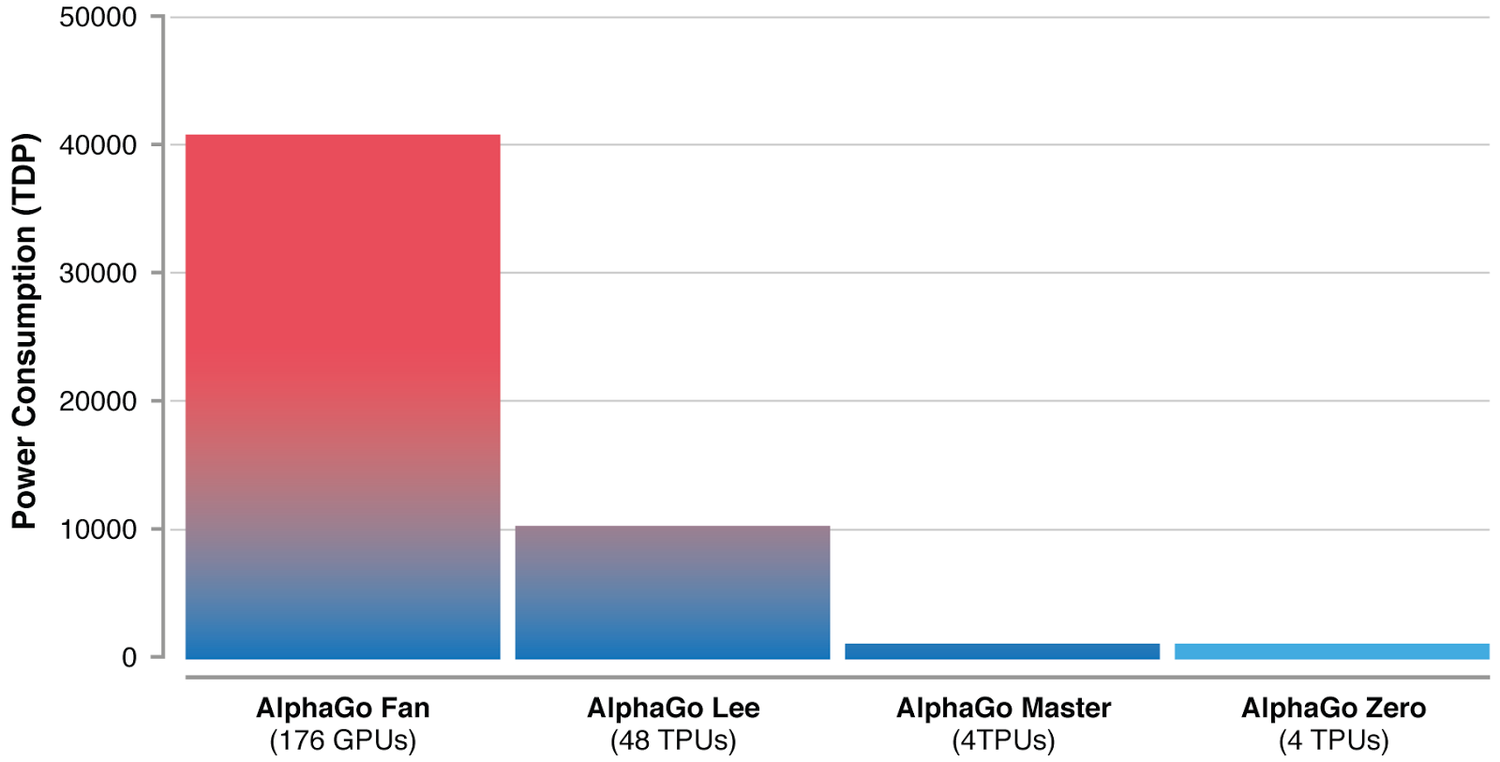
\includegraphics[width=\textwidth]{figures/rl/alphago_power.png}
				\caption{AlphaGo Versions Compute Power}
				\label{fig:alphago_power}
		\end{subfigure}
		\hfill

		\begin{subfigure}[b]{0.3\textwidth}
				\centering
				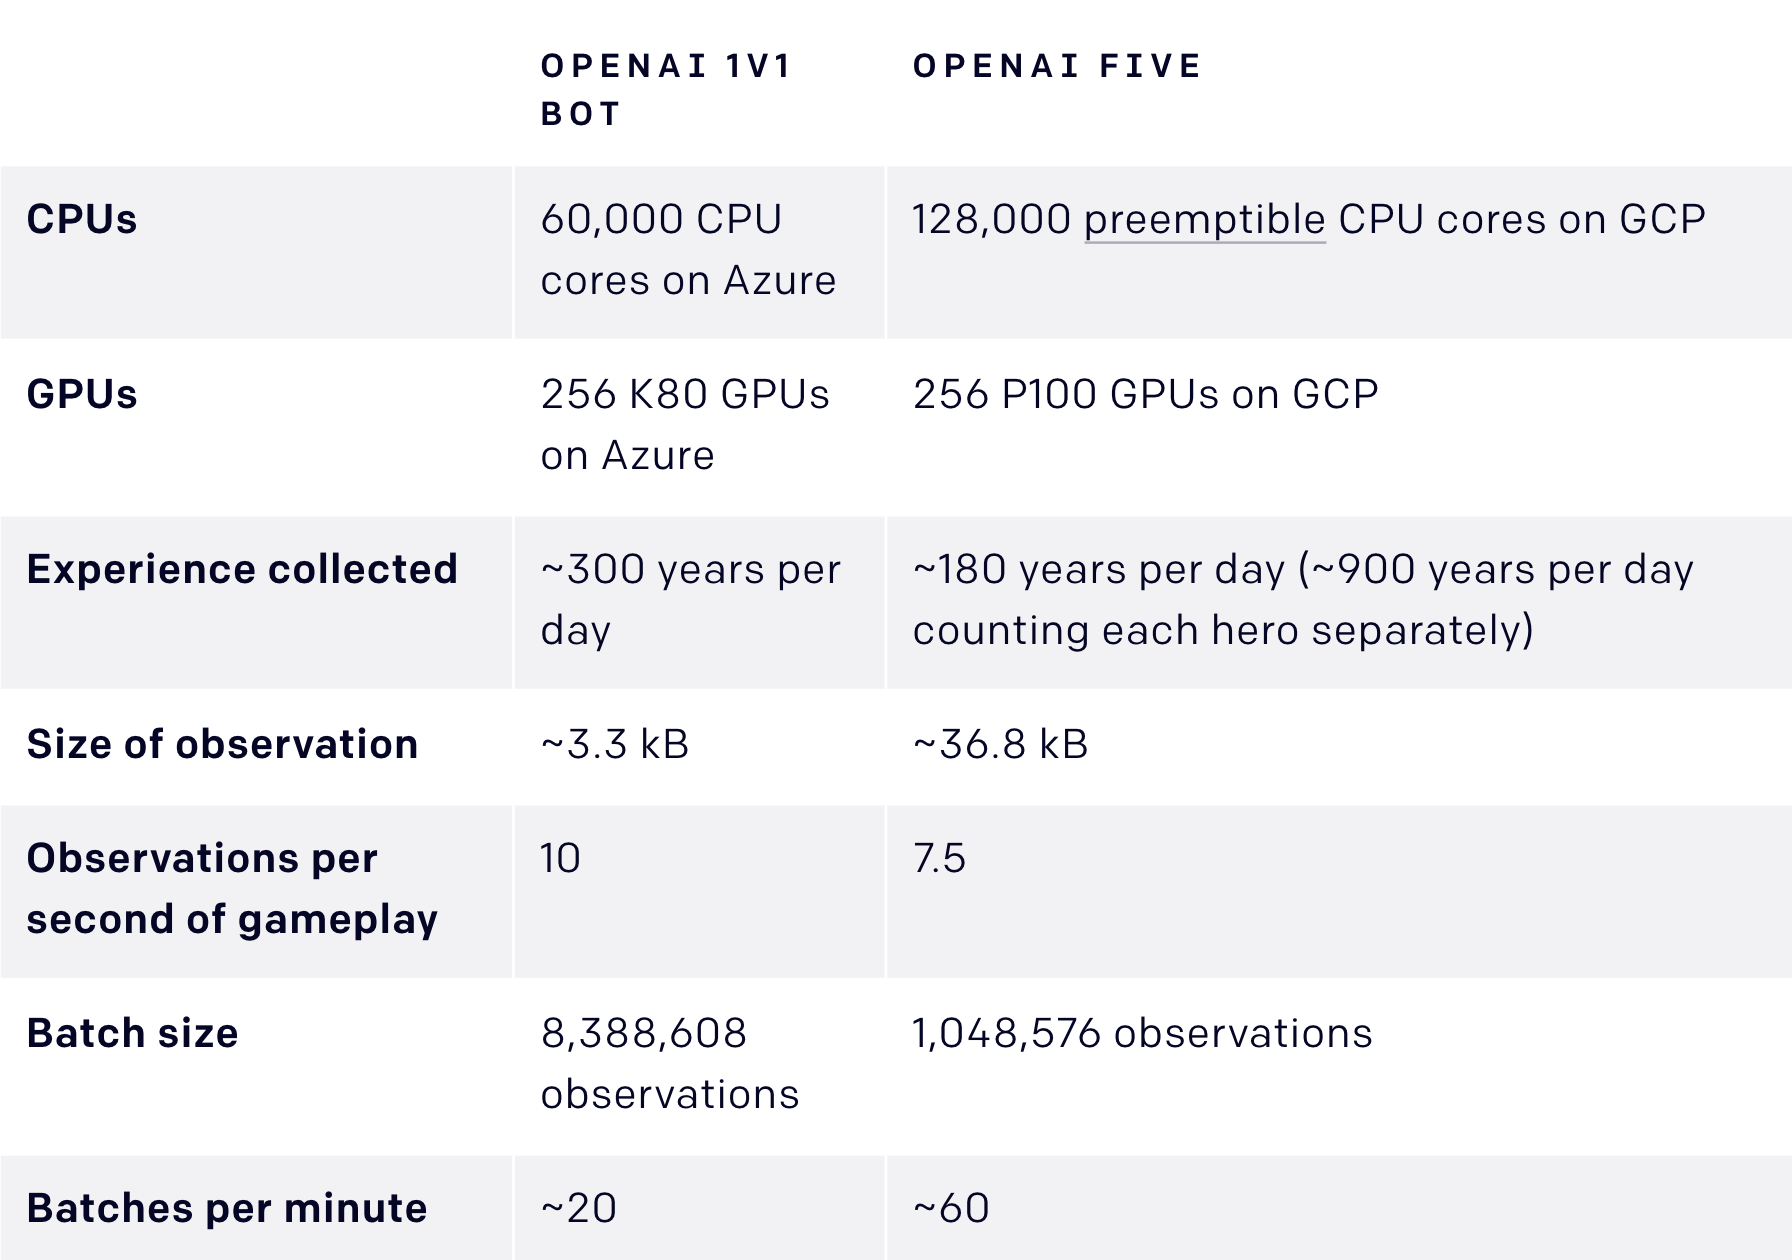
\includegraphics[width=\textwidth]{figures/rl/openai_five_hardware.png}
				\caption{Hardware used for OpenAI Five}
				\label{fig:five_hardware}
		\end{subfigure}
		\hfill
		\begin{subfigure}[b]{0.3\textwidth}
				\centering
				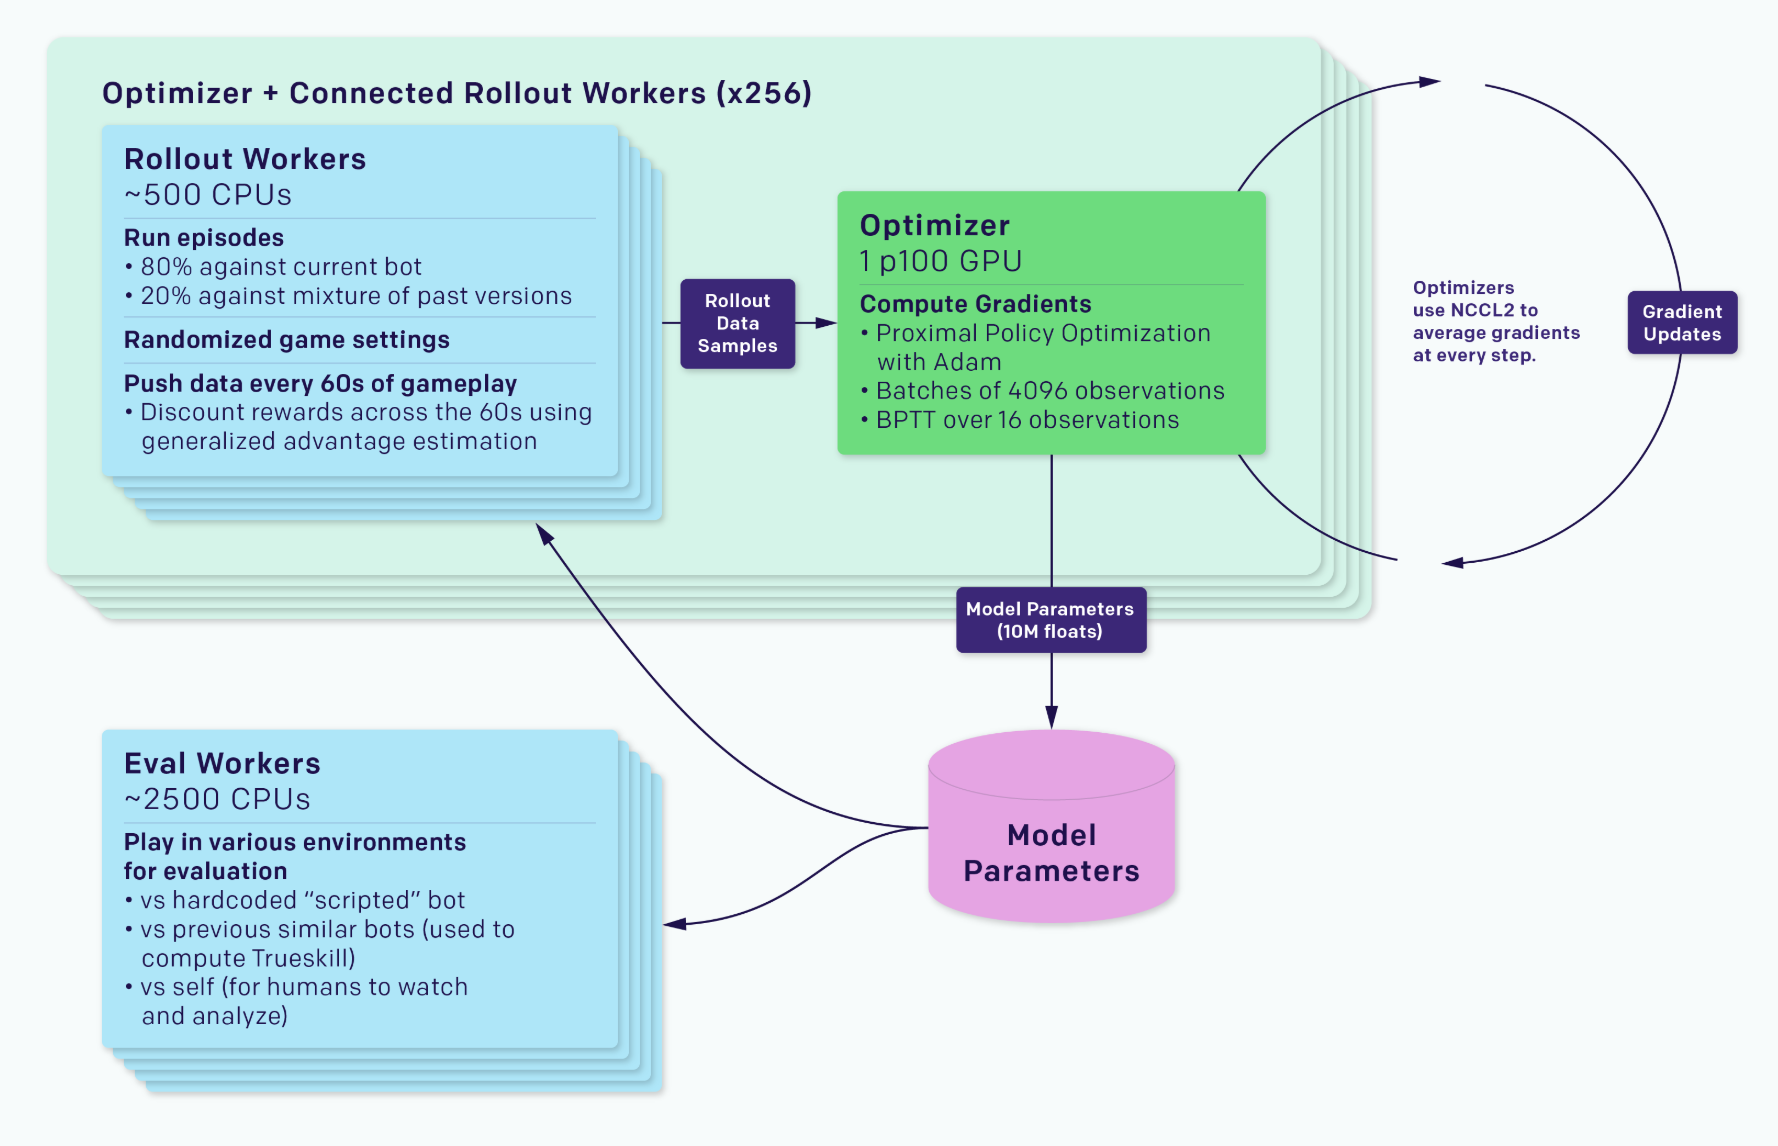
\includegraphics[width=\textwidth]{figures/rl/openai_five_training.png}
				\caption{OpenAI Training Workflow}
				\label{fig:openai_five_training}
		\end{subfigure}
		\hfill
		\begin{subfigure}[b]{0.3\textwidth}
				\centering
				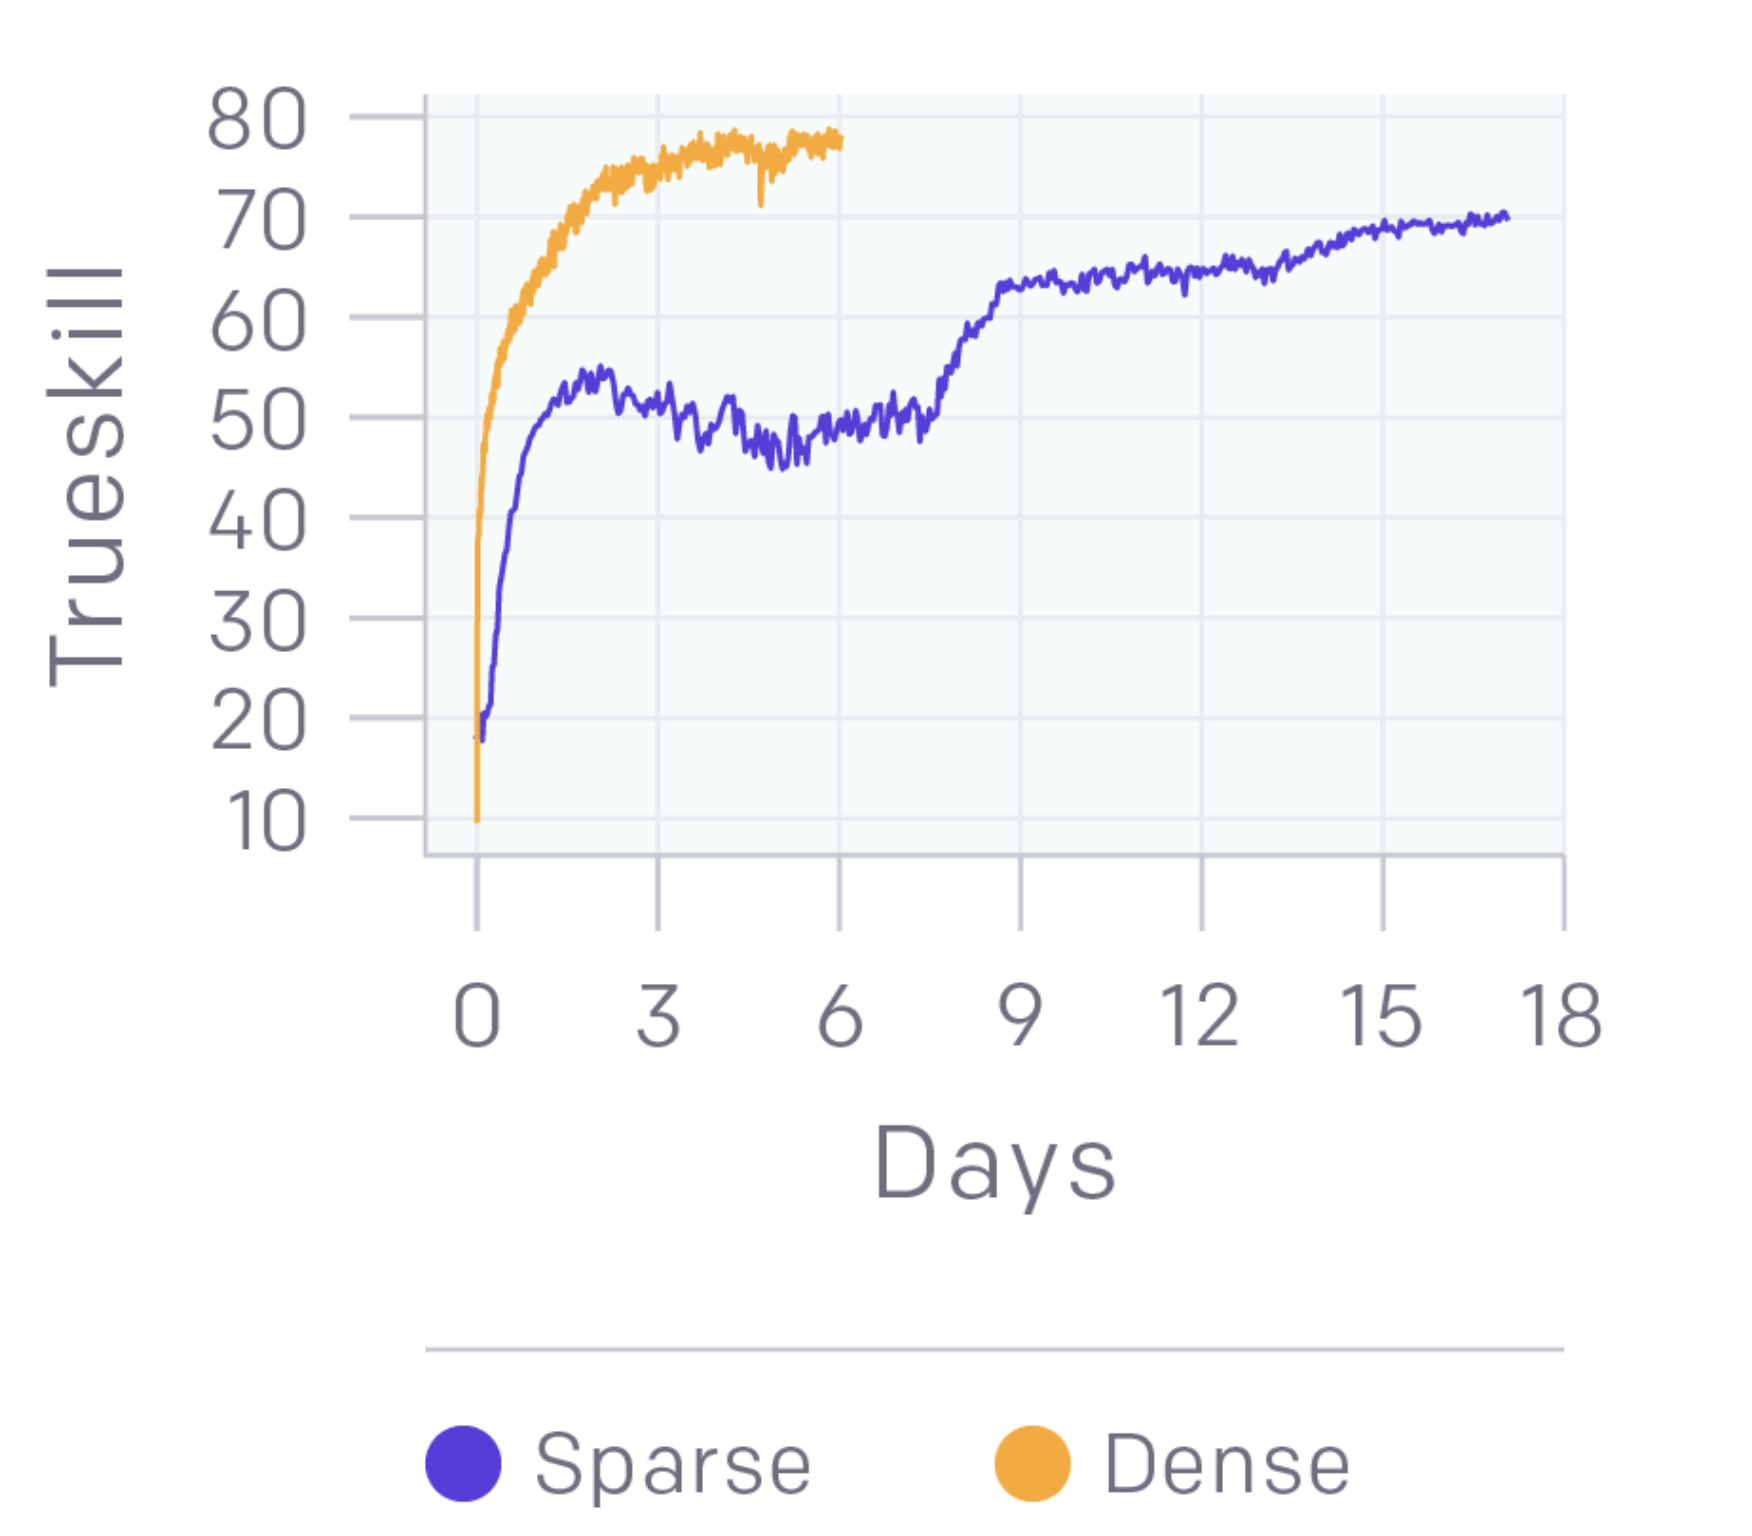
\includegraphics[width=\textwidth]{figures/rl/openai_five_time.png}
				\caption{OpenAI Training Time}
				\label{fig:openai_five_time}
		\end{subfigure}
		\hfill
		 \caption{AlphaGo Zero \& OpenAI Five}
		 \label{fig:zero_and_five}
\end{figure}

This introduces a critical \textit{\textbf{(experiment turn-around time)}} bottleneck for reinforcement learning research and in practice along with key issue to design algorithms that are both scalable and data-efficient. To overcome this bottleneck, new approaches and directions are being followed towards using distributed setups toward accelerating reinforcement learning experiments, reduce the training time, and scales the algorithms effectively. Hence, reinforcement learning needs to support fine-grained computations and render actions in milliseconds when interacting with the real world or performing vast numbers of simulations. It has to support utilizing the resources usage and support heterogeneity in time for both simulation time which takes milliseconds or hours and the GPUs and CPUs wall-time for simulations. Also, supporting dynamic execution, as results of simulations or interactions with the environment can change future computations. 

This leads the way to build new frameworks and investigating how to optimize existing reinforcement learning algorithms for modern computers, to better leverage usage of multiple CPUs and GPUs and the combination between them, providing the proper scalability and utilizing distributed training.

Recently, there have been a quite interest and research on the scalability and distribution of RL algorithms and training with a parallel and different environment to enhance the performance of the agents and reduce the amount of time it takes to master the learning task.

\section{Objectives}
In this research project, the aim is to train and test a set of reinforcement learning algorithms to different reinforcement learning environments and run experiments in non-distributed setup vs parallel and distributed setup to measure the effect on the training process and compare the performance among these environments and see the effect of the distribution and the power of using and utilizing multiple CPUs and GPUs setup. 

We will be comparing the state of the art algorithms mentions in the related work section~\ref{related_work} using Ray framework as our backend for the experiments along with some of the implemented algorithms. We created our abstract class to unify the differences between RL environments providing simplicity and clarity to deal with the environments and to be easy to use with other existing frameworks.

Then with our distributed learning architecture and setup we provide evaluation for distribution and transferability of networks between different physics simulators with full benchmarking for all the experiments we have done along with comparisons between all of the environments and applied algorithms.

\section{Overview and Outline}
The work is organized as follows. In \autoref{chapter:background_and_foundations}, the theoretical background linked to reinforcement learning and the Markov decision process framework are introduced. Furthermore, we discuss the use of deep learning in the RL framework and the state of the art algorithms. Finally, we discuss the related work and existing distributed framework. The \autoref{chapter:methodology} presents the task description, the setup of our experiments with the architecture, frameworks, and classes used to accomplish our research goal. \autoref{chapter:experiments} illustrate the experiments we have done along with the results and comparisons. Finally, \autoref{chapter:conclusion_and_future_work} summarizes the work, discusses future work and concludes.
